% \externaldocument{0_frontmatter/abbreviations.tex}
\section{Systems Dynamics}
\label{sec:sysdyn}
The modern understanding of biology has grown concomitantly with the means and methods by which to characterize deeper and with more resolution the various biological levels of organization, \eg tissues, cells, organelles, protein structures, \etc. This is made possible, in part by developments in biophysics and biochemistry which usher in ever more fine grained probing technologies \cref{sec:bioreg}. Similarly, the interdisciplinary field of systems biology has borrowed many tools from the domains of mathematics and physics. For example, the study of complex systems lends to analysis of \emph{emergent} organizational structure leading to function which cannot be explained by investigating individual constituent components alone. In biology, a systems approach is needed to track the many collective, macroscopic effects individual interacting components spontaneously birth. Derived from the latin \emph{plexus} meaning intertwined, the ying to complexity's yang is separability. Reducing complex systems to components removes novel information regarding interaction and thus limits predictive capabilities on that same system. This is a major motivation for inferring the network at once using ordinary differential equations (ODE) rather than many mutual information (MI) methods which infer links individually in relation to one another, discussed in \cref{sec:info}. Furthermore, our group has found several data properties to be strong indicators of the ability to correctly, accurately and reproducibly infer networks. The following offers a brief introduction to these relevant attributes as we have defined them, including sparsity in \cref{sec:spar}, the signal-to-noise ratio in \cref{sec:snr}, and condition number or Interampatteness in \cref{sec:cond}.


\subsection{Two General Strategies}
\label{sec:purpose}
In the landmark paper of its kind, Gardner and Faith \citep{gardner2005reverse}, and later reviewed \citep{HECKER200986}, offer descriptions of types of networks based on two aims. The first offers a \emph{physical} view of direct binding interactions among biomolecules via chemical or other linkages. To leave a single biomolecule unquantified risks its activity being interpreted as that of another molecule, and thus this method is both highly expansive scope as well as rather dubious to characterize. Thus, a second \emph{influential} approach is proposed, whereby indirect interactions are allowed by the added caveat that any measured interaction is necessarily not-direct. This type of network contains interactions capable of passing through innumerable intermediate biomolecules and indeed levels of biology on its way to affecting its eventual target. A major assumption of this research lies in the nature of the response to perturbation, \ie that the system has reached some state whereupon interaction between genes is stable and major change is less likely \citep{gardner2003inferring, gardner2005reverse,tegner2003reverse}. This surely simplifies reality but is quite powerful for modeling the large, overriding tendencies driving operations crucial to cellular life, and as such has seen extensive adoption in the field of biology including the clinic \citep{kusko2016integrated}.  These works form the foundation of the work and many of the ideas presented here. 


\subsection{Regulation is as much about \emph{what} as it is about \emph{when}}
\label{sec:regwhatwhen}
Dynamics is in its most basic form a study of what and when -- by how much has any given system element changed over any given element of time. Determining these rates of change is the primary concern of experimental biologist wishing to better understand their investigative niche, for example. Together these niche experts can bind their individual biomolecules of interest together into a system using equations defining their rates of change in relation to one another using a \emph{system of equations}. As with all models, there is a trade-off between the accuracy of your model and the complexity. The simpler the equations, \ie the fewer parameters and lower the complexity, the fewer degrees of freedom and by extension the fewer data points are needed to recreate the observed behavior compared to the more complex alternative. However, description of the given system can vary in appreciable ways depending on the modeling paradigm adapted. 
\emph{Nonlinearity} presents the potential for higher resolution, but risks misrepresenting underlying biology by overfitting to input data. Systems by definition are closed, and as such, stability is born in the balance of growth and death, where degradation prevents system-wide collapse due to runaway growth\citep{alon2007design}. This can be carried out through feedback or feed forward (see \cref{sec:pat}), alerting the system to the dangers of blindly continuing its present course without adaptation. Nonlinear models might be especially useful for modeling the robust capabilities of many natural systems to host multiple stable, \emph{steady states}, where overall change is null, \eg modeling diauxic growth of \coli on glucose and lactose \citep{wong1997mathematical} where the model must encompass for similar growth function under the presence of separate metabolite, see \cref{sec:stab}. 
Work has also been done to show that nonlinear systems, in which there is no proportional relationship between a given input and its effect on the systems output, can be approximated fairly well using the simpler linear models when the system finds a single steady state \citep{wildenhain2006reconstructing, crampin2006system,zavlanos2011inferring}.  \emph{Linear} relationships enable simplification at the cost of reflecting abstractions of truth. Simplifying the exemplified model to linearity might mean diminishing focus on individual metabolite levels and simply accounting for survival, \eg noting any lag period indicative of the bacterium trying to adjust to any limited resource before initiating death phase.


\subsection{Parameter Estimation}
\label{sec:parest}
A prerequisite to modeling any system is a means of mapping two sets of variables to one another. Convention dictates this function use various assemblies of parameters to equate independent and dependent variables. Thus we implement a linear model to determine the parameter values which will fit observed data to model outputs. Here our investigation is focused on changes in gene expression over time, and thus an element of time must be incorporated, making our models dynamic via implementation as \emph{first-order} linear differential equations, \ie relying on the function's first derivative. Also, because the quantity we strive to characterize is dynamic, \ie deviates over time, compounded by the fact that the measurements we gather are prone to error, elements of noise persist into our data. Thus an estimation of noise is calculated for, as follows:

\begin{equation}
\label{eq:Linearmap}
  Y = -A^{-1}(P+F)+ E,
\end{equation}
% \myequations{Linear Map}

where the independent measurements Y map to the known experimental design P to solve for a GRN structure, A, which explains both while also accounting for systematic and model error, E \& F. As such, the rate of change defining the system's assumed steady state (after perturbation) is calculated as the sum effect of all other regulators for the gene. The model parameters we are solving for facilitate the mapping of variables to one another as defined by our input measurements, \ie an inverse problem, which we resort to solving using modern methods. Many methods can solve this problem, but an optimal minimum-variance, unbiased estimator (MVUE) for sufficiently large datasets remains largely elusive \citep{kay1993fundamentals}. As such, presented next are several methods which compete for the title of least bias and most accuracy. As one may guess, there are trade-offs between them which require the survival of the others, \ie no universal winner \citep{marbach2010revealing,narendra2011comprehensive}.



\subsection{Regression}
\label{sec:regress}
Gauss first devised the least squares estimation to study planetary motion in the late 18th century. Simply put, one uses regression analysis to see how a dependent variable changes with respect to an independent variable. Linear models such as \emph{least squares} suffice in predicting relationships between input and output variables reasonably well, especially in cases of small sample size, low SNR (see \cref{sec:snr}) or sparse data (see \cref{sec:spar}){friedman2001elements}. Such makes this \emph{elementary} approach particularly well suited here in this biological context. This carries known limitations, namely returning estimates with large variance and large state space, \ie accounting for variables which are not necessary to describe the ``big picture''\citep[p.57]{friedman2001elements}. However, least squares (LS) and our implementation have been improved upon using \emph{pseudo-inverse} functionality \citep{carlson1974generalization} to enable operating at such sparsities as GRN require. Additionally, this has been fit with an added constraint, a cutoff (LSCO) \cref{eq:LSCO}, where sparsity is given to the solution \emph{post hoc} in a stepwise manner determined by link confidence.

When fitting the data to the perturbation matrix with an estimated error on each, we seek to minimize the difference, the distance between the matrices, as in our linear model presented in \cref{sec:ODE}. Here we find Gauss' ideas and methods it has inspired similarly valid \emph{regression} approaches (\cref{eq:LSCO} and a total LSCO (TLSCO) variant \cref{eq:TLSCO} \citep{de1998introduction} which carries out this minimization along both independent and dependent variables) to minimize the residuals between the experimental measurements and the line when estimating parameters in our model (\cref{eq:Linearmap}).

%  \begin{subequations}
  \begin{equation}
       \hat{A}_{LS}={{Y^TY}^{-1} Y^TP} > \zeta
 \label{eq:LSCO}
 \end{equation}

\begin{equation}
  \begin{aligned}
%     \svd
    \lbrack Y P\rbrack &= U S V , \\
    \hat{A}_{TLS} &= -\frac{VYP}{VPP} > \zeta
 \label{eq:TLSCO}
 \end{aligned}
 \end{equation}

Here $\zeta$ is cutoff based on link confidence below which links are not included, thus returning variously sparse GRN. Recently, issues of scaling have since arisen as we have pushed to include more genes into our GRN. Specifically, we have hypothesize the lack of regularization in our LSCO implementation, which has led to our reliance on LASSO, described in \cref{sec:reg}, begets mega-hub regulator genes unrealistic in biologic systems \cref{fig:hubiness} \citep{bock2012hub}. While there is undeniable bias in both methods, the extent to which LASSO creates unwarranted hubs of degree 30 is 10 fold less than that of LSCO at degree 250+. This is an ongoing and quite interesting problem to have stumbled upon, and results are unpublished. While the results are quite conclusive and broad-spanning (both in cases of synthetic and real datasets), no solution has yet been implemented.

\begin{figure}[H]
\centering
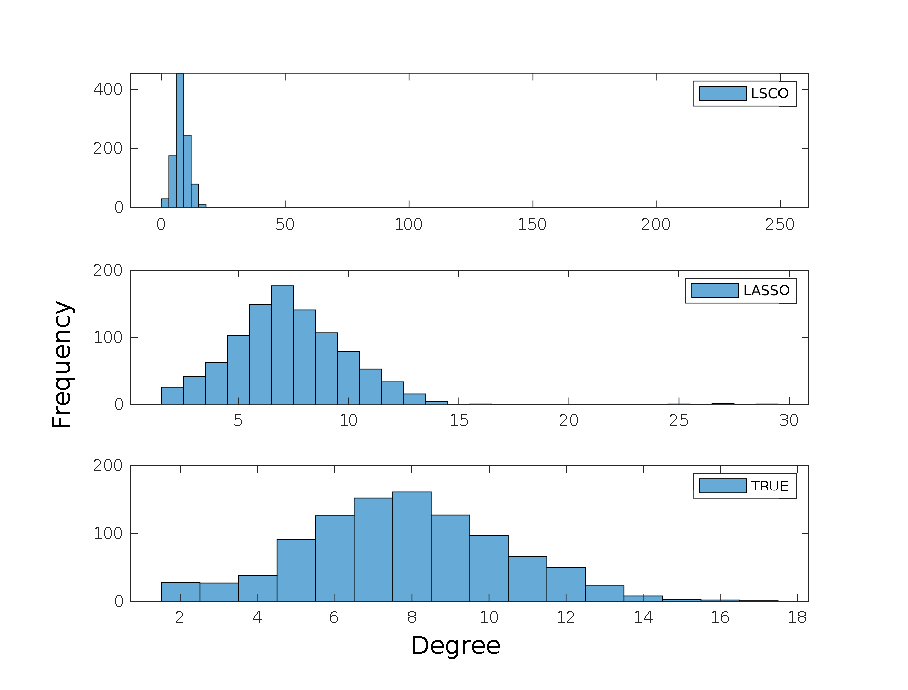
\includegraphics[width=1\linewidth]{3/hubs.eps}
\caption{\textbf{GRN node degree distributions per method.} A synthetic 1000 gene (N) network was created, where the true sparsity is $\zeta$=3.89, data synthesized and GRN inferred using both LSCO and LASSO, with sparsities chosen to match this truth as close as possible, at $\zeta$=3.978 and $\zeta$=3.676, respectively.}
\label{fig:hubiness}
\end{figure}




% Linear ODE- Least squares with penalty
% LASSO/ridge (L1,L2), Elastic net
\subsection{Regularization, OR penalized Regression}
\label{sec:reg}
Similar in aim but more capable when confronted with collinearity or seeking sparse solutions, several competing \emph{regularization} approaches exist, each with strengths, which under the right circumstances may outweigh any limitations \citep[p.69-73,661-668]{friedman2001elements}. LASSO (short for (least absolute shrinkage and selection operator) (\cref{eq:linLASSO},\citep{tibshirani1996regression}), Ridge Regression (also known as Tikhonov regularization, \cref{eq:ridge} \citep{hoerl1970ridge}) and Elastic-Net (El-Net) (\cref{eq:EL}\citep{zou2005regularization}) are, in effect, similar but distinct ways of minimizing this distance between matrices when regressing, summarized in \cref{table:regularization}. LASSO somewhat erratically picks one variable over the other, while Ridge Regression shrinks them towards one another for a more consistent, reproducible result \citep{ng2004feature,tibshirani1996regression}. Seeking a middle group, Elastic-Net seeks to exploit strengths of both to overcome their individual weaknesses.

 \begin{equation}\label{eq:linLASSO}
 %\argmin_{\mA} \frac{1}{2m} \norm{\mA_i\mY^T+\mP^T_i}^2_F + \zeta \norm{\mA}_1 %\citep{Glmnet-LASSO}
  \hat{A}_{\textrm{LASSO}}(\tilde{\zeta}) = \arg \min_{A} ||A Y+P||^2_{L_2} + \tilde{\zeta} ||A||_{L_1},
\end{equation}

 \begin{equation}\label{eq:ridge}
  \hat{A}_{\textrm{Ridge}}(\tilde{\zeta}) = \arg \min_{A} ||A Y+P||^2_{L_2} + \tilde{\zeta} ||A||^2_{L_2},
\end{equation}

 \begin{equation}\label{eq:EL}
  \hat{A}_{\textrm{El-Net}}(\tilde{\zeta}) = \arg \min_{A} ||A Y+P||^2_{L_2} + \tilde{\zeta} ||A||_{L_1}+ \tilde{\zeta} ||A||^2_{L_2},
\end{equation}

Whereas least squares \cref{eq:LSCO} returns an estimate of fit for all variables which results in models which suffer from poor generalizability or issues of over fitting, regularization methods use a penalization regulated by the parameter $\zeta$ to solve \emph{ill-posed} (see \cref{sec:calc}) problems such as our inverse problem of inferring GRN from expression and design matrices. The implementation of zeta in methods herein returns variously sparse networks, and so can equally be thought of as a sparsity parameter (see ~\nameref{nom}). Choosing the right model returned by LASSO or Elastic-Net then becomes a game of comparing predictions to some ground truth, usually left-out training data, \ie via cross validation referenced in \cref{sec:calc} and \cref{sec:acc}.

\begin{table}[H]
\begin{tabular}{|l|l|l|l}
\cline{1-3}
 & \textbf{LASSO} &  \textbf{Ridge} &  \\ \cline{1-3}
\textit{norm} & L1 &  L2 &  \\ \cline{1-3}
\textit{selection} & sparse  & shrinks &  \\ \cline{1-3}
\textit{scaling} & not independent &  independent &  \\ \cline{1-3}
\textit{constraint} &sum of absolute coefficients& sum of squared differences&  \\ \cline{1-3}
\textit{penalization} & more uniform &  larger preferred &  \\ \cline{1-3}
thresholding & soft &  hard &  \\ \cline{1-3}
\end{tabular}
\caption{Comparison among L1 and L2 regularization techniques}
\label{table:regularization}
\end{table}

\subsection{Calculability}
\label{sec:calc}
Several methods exist for solving minimizations problems, not limited to those listed in \crefrange{eq:LSCO}{eq:EL}, however unique parameter estimations are not guaranteed \citep{candes2009near}. Such cases are denoted \emph{underdetermined} and deemed \emph{nonidentifiable}; here the specific case of inverse problem solving returning non-unique solutions requires additional assumptions, \ie are \emph{ill-posed} problem. Both biological and technical replicates can help to decrease uncertainty in such estimates \citep{lee2000importance}. Furthermore, biological replicates enhance the utility of \emph{bootstrapping} by expanding the creative potential for new datasets to estimate parameters. Assuming any systemic noise is both uniform and independent, such repeated experiments offer estimations of both true variability of the biological system as well as of noise implicit to the characterization system. Disambiguating these quantities is not trivial. Thus, expanding the number of measurements in the form of \emph{resampled} datasets is one way to improve the parameter estimation, returning a better estimate of the parameter space. However, the model loses its ability to generalize, \ie to reliably predict new data, especially when points are missing \citep{folch2015enabling}, when more data is used for parameter estimation as the risk of overtuning arises. For this reason, a simple solution can be made by removing portions of individual datasets, training on only a random portion, which you shuffle around across many calculations. Such \emph{cross validation} techniques are widely used in modern \emph{machine learning} practices. A caveat to such practice, however, is that by requiring more calculation, more time is often require. Depending on the underlying estimation efficiency (LSCO \cref{eq:LSCO} compared to something like LASSO \cref{eq:linLASSO}), this can amount to quite large increase overall compute time.


\subsection{Network Inference}
\label{sec:netinf}
Networks arrange information regarding the interactions of constituent members in a manner prone to statistical analysis and often aid in human understanding. In the context here, a node is generally in reference to a singular biomolecule, be it transcription factor, gene, intermediate gene product, protein, \etc, which plays some role in the regulation of another such factor. Regulation comes about by a binding interaction of some sort dictated by the level of biology. This relational information is conveyed as a weight, the degree to which one factor influences another, and can either convey up- or down- regulation.

Several approaches exist for this reverse engineering, ranging from an outdated assembly of one-to-one relationships to correlating patterns throughout expression assays, \etc. Some inference methods return link existence with no confidence or weight, so called \emph{binary networks} (see \cref{sec:models}). In this and other scenarios, link weights can be estimated after link existence is establish. Such was the case after the creation of a null inferred network distribution, as in \textbf{Paper II}. In that study, however, struggling to find a representative null distribution realistic enough to compare to and thus implement an FDR restriction, we refit inferred, shuffled network links using constrained least squares (CLS, \cref{eq:CLS}, \citep{grant2008cvx} in the context of \cref{eq:Linearmap}) to improved their performance against measured links (detailed in the authors note in \cref{note}). 


\begin{equation}%\label{eqn:CLS}
\begin{aligned}\label{eq:CLS}
  \hat{A} = \arg min_{A} & \sum \diag(\Delta^TR \Delta), \\
  \text{s.t.}\; & \Delta = A Y + P, \\
% \label{eqn:CLSPredErr} \\
  & R = \left( \hat{A}_{\textrm{init}} \Cov[y] \hat{A}_{\textrm{init}}^{T} + \Cov[p]\right)^{-1},\\ %\label{eqn:CLSR} \\
  & \sign{A} = \sign{\hat{A}_{\textrm{reg}}}. \\
%   \label{eqn:CLSStructure}
\end{aligned}
\end{equation}
% \myequations{CLS}

This process is contained within the general ``BalanceFitError" algorithm in \textbf{Paper III}, wherein this optimization is iterated for balancing among input and output errors. This is done in order to minimize the overall error of the network reproducing the dataset in a leave-out manner, while still accounting for error inherent to the creation of the perturbation design matrix used in our linear model (\cref{eq:Linearmap}).

\subsection{Comparison to Null: Limiting Random Artifacts}
\label{sec:null}
The novelty and power of both \textbf{Paper II} and \textbf{Paper III} is drawn from a comparison to a null distribution of shuffled data and shuffled links, respectively. Networks inferred from shuffled data offer an estimate of how likely it is by chance to retrieve any given link by random chance. Constructing a consensus network in comparison to these random-chance links as we did thus restricts links from inclusion. These links likely constitute false links, and as such inclusion in the final network would do so at the cost of increasing the \emph{false discovery rate} (FDR) \citep{kall2007posterior}. In a similar way, testing how well shuffled GRN reproduce independent datasets allows testing of significance of how well a GRN inferred from real data can do the same. These null distributions are admittedly na{\"i}ve, but nevertheless have been shown to provide real improvement through their implementation in various pipelines here and elsewhere. Specifically, note such a null distribution is constructed from $10^5$ permuted label versions in the chronic obstructive pulmonary disease (COPD) case study \citep{platig2016bipartite} for a similar comparison, lending significance to Genome Wide Association Studies (GWAS) SNP data used to infer regulatory relationships between and among genes (see \cref{sec:practical}).